\documentclass{article}

\usepackage{graphicx}
\usepackage{tikz}
\usepackage{tikzsymbols}
\usetikzlibrary{calc,patterns,shapes.geometric}
\pagestyle{empty}
\usepackage[margin=0pt]{geometry}
\geometry{papersize={14in,12in}}

\def\centerarc[#1](#2)(#3:#4:#5){\draw[#1] ($(#2)+({#5*cos(#3)},{#5*sin(#3)})$) arc (#3:#4:#5);}

\begin{document}
	\begin{figure}
		\centering
		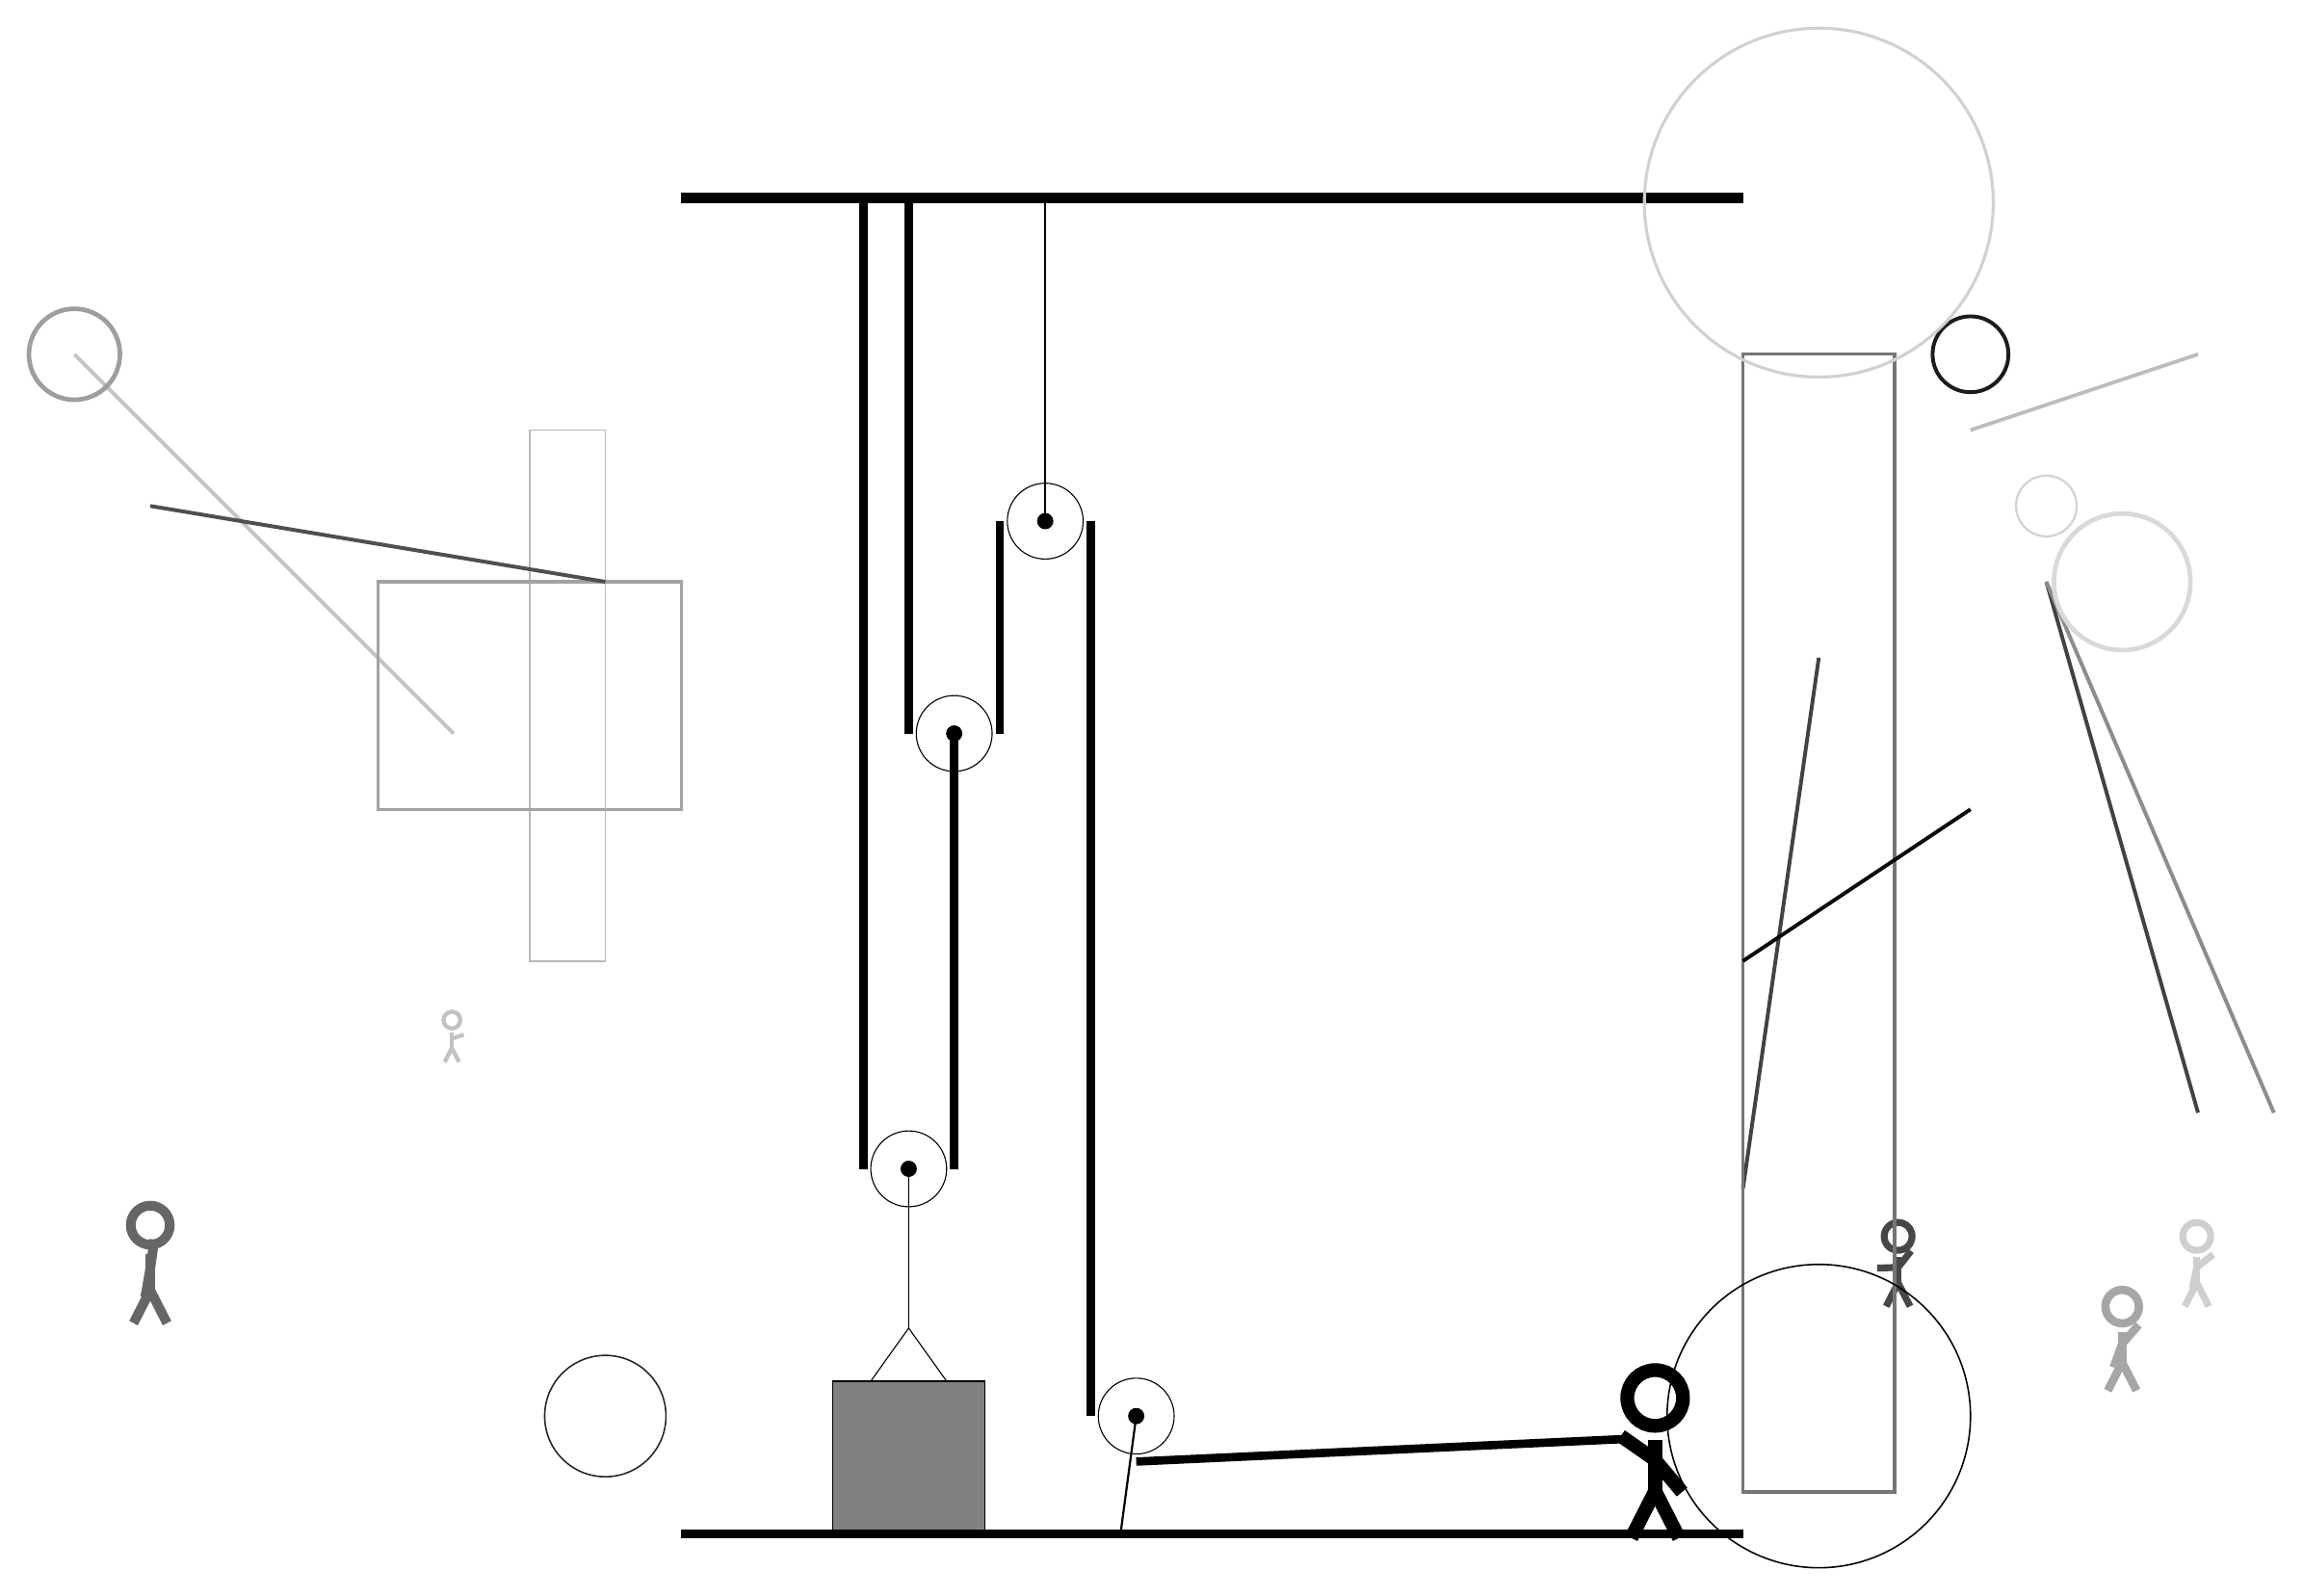
\begin{tikzpicture}
			%%%%% START %%%%%
			
			\draw[fill=black] (-2, 14) rectangle (12, 14.125);
			
			\draw (1, 1.26) circle (0.5);
			\draw[fill=black] (1, 1.26) circle (0.1);
			
			\draw[line width=0.5mm, color=black!26](15, 11) -- (18, 12);
			
			\node[line width=0.7mm, color=black!60] at (-9, 0) {\Strichmaxerl[7][80][82]};
			\draw [line width=0.7mm, color=black!59](-7, 9) circle (0.0);
			\draw [line width=0.5mm, color=black!89](15, 12) circle (0.5);
			
			\draw[line width=0.5mm, color=black!23](-5, 7) -- (-10, 12);
			\node[line width=0.7mm, color=black!35] at (17, -1) {\Strichmaxerl[6][70][49]};
			\draw[line width=0.5mm, color=black!74](13, 8) -- (12, 1);
			
			\draw[line width=0.5mm, color=black!74](16, 9) -- (18, 2);
			\node[line width=0.4mm, color=black!72] at (14, 0) {\Strichmaxerl[5][2][52]};
			
			\draw [line width=0.6mm, color=black!38](-10, 12) circle (0.6);
			\draw[line width=0.2mm, color=black!28] (-3, 4) rectangle (-4, 11);
			\draw[line width=0.4mm, color=black!36] (-2, 6) rectangle (-6, 9);
			\draw[line width=0.4mm, color=black!54] (14, -3) rectangle (12, 12);
			\draw[line width=0.5mm, color=black!69](-3, 9) -- (-9, 10);
			\node[line width=0.5mm, color=black!19] at (18, 0) {\Strichmaxerl[5][78][38]};
			\draw [line width=0.3mm, color=black!17](16, 10) circle (0.4);
			
			\draw [line width=0.4mm, color=black!18](13, 14) circle (2.3);
			\draw[line width=0.5mm, color=black!45](16, 9) -- (19, 2);
			\draw[line width=0.5mm, color=black!96](12, 4) -- (15, 6);
			
			\draw [line width=0.2mm, color=black!85](-3, -2) circle (0.8);
			\node[line width=0.2mm, color=black!24] at (-5, 3) {\Strichmaxerl[3][90][19]};
			
			\draw [line width=0.2mm, color=black!99](13, -2) circle (2.0);
			\draw [line width=0.6mm, color=black!15](17, 9) circle (0.9);
			
			\draw (1.6, 7.0) circle (0.5);
			\draw[fill=black] (1.6, 7.0) circle (0.1);
			
			\draw (2.8, 9.8) circle (0.5);
			\draw[fill=black] (2.8, 9.8) circle (0.1);
			\draw[thick] (2.8, 9.8) -- (2.8, 14);
			
			\draw (4.0, -2) circle (0.5);
			\draw[fill=black] (4.0, -2) circle (0.1);
			\draw[thick] (4.0, -2) -- (3.8, -3.5);
			
			\draw (1, 1.26) -- (1, -0.84) -- (0.5, -1.54) -- (1.5, -1.54) -- (1, -0.84);
			\draw[fill=black!50] (0, -1.54) rectangle (2, -3.54);
			\draw[line width=1.1mm] (0.4, 14) -- (0.4, 1.26);
			\centerarc[line width=1.1mm](1, 1.26)(180:360:0.6);
			\draw[line width=1.1mm](1.6, 1.26) -- (1.6, 7.0);
			\draw[line width=1.1mm] (1.0, 14) -- (1.0, 7.0);
			\centerarc[line width=1.1mm](1.6, 7.0)(180:360:0.6);
			\draw[line width=1.1mm](2.2, 7.0) -- (2.2, 9.8);
			\centerarc[line width=1.1mm](2.8, 9.8)(0:180:0.6);
			\draw[line width=1.1mm] (3.4, 9.8) -- (3.4, -2);
			\centerarc[line width=1.1mm](4.0, -2)(0:90:-0.6);
			\draw[line width=1.1mm](4.0, -2.6) -- (10.5, -2.3);
			
			\node at (10.8, -2.5) {\Strichmaxerl[10][-35][-50]};
			
			\draw[fill=black] (-2, -3.5) rectangle (12, -3.6);
			
			%%%%% END %%%%%
		\end{tikzpicture}
	\end{figure}	
\end{document}